
\documentclass{beamer}

\usepackage{algpseudocode}

\usetheme{Montpellier}
\usecolortheme{rose}

% page numbers, from
% https://tex.stackexchange.com/questions/137022/how-to-insert-page-number-in-beamer-navigation-symbols
\expandafter\def\expandafter\insertshorttitle\expandafter{%
  \insertshorttitle\hfill%
  \insertframenumber\,/\,\inserttotalframenumber}

\newcommand{\stanza}{ \\~\ }

\title{03. Divide-and-Conquer}
\subtitle{CPSC 535}
\author{Kevin A. Wortman}
\institute{ 
\includegraphics[height=2cm]{csuf-logo-cmyk} }
\date{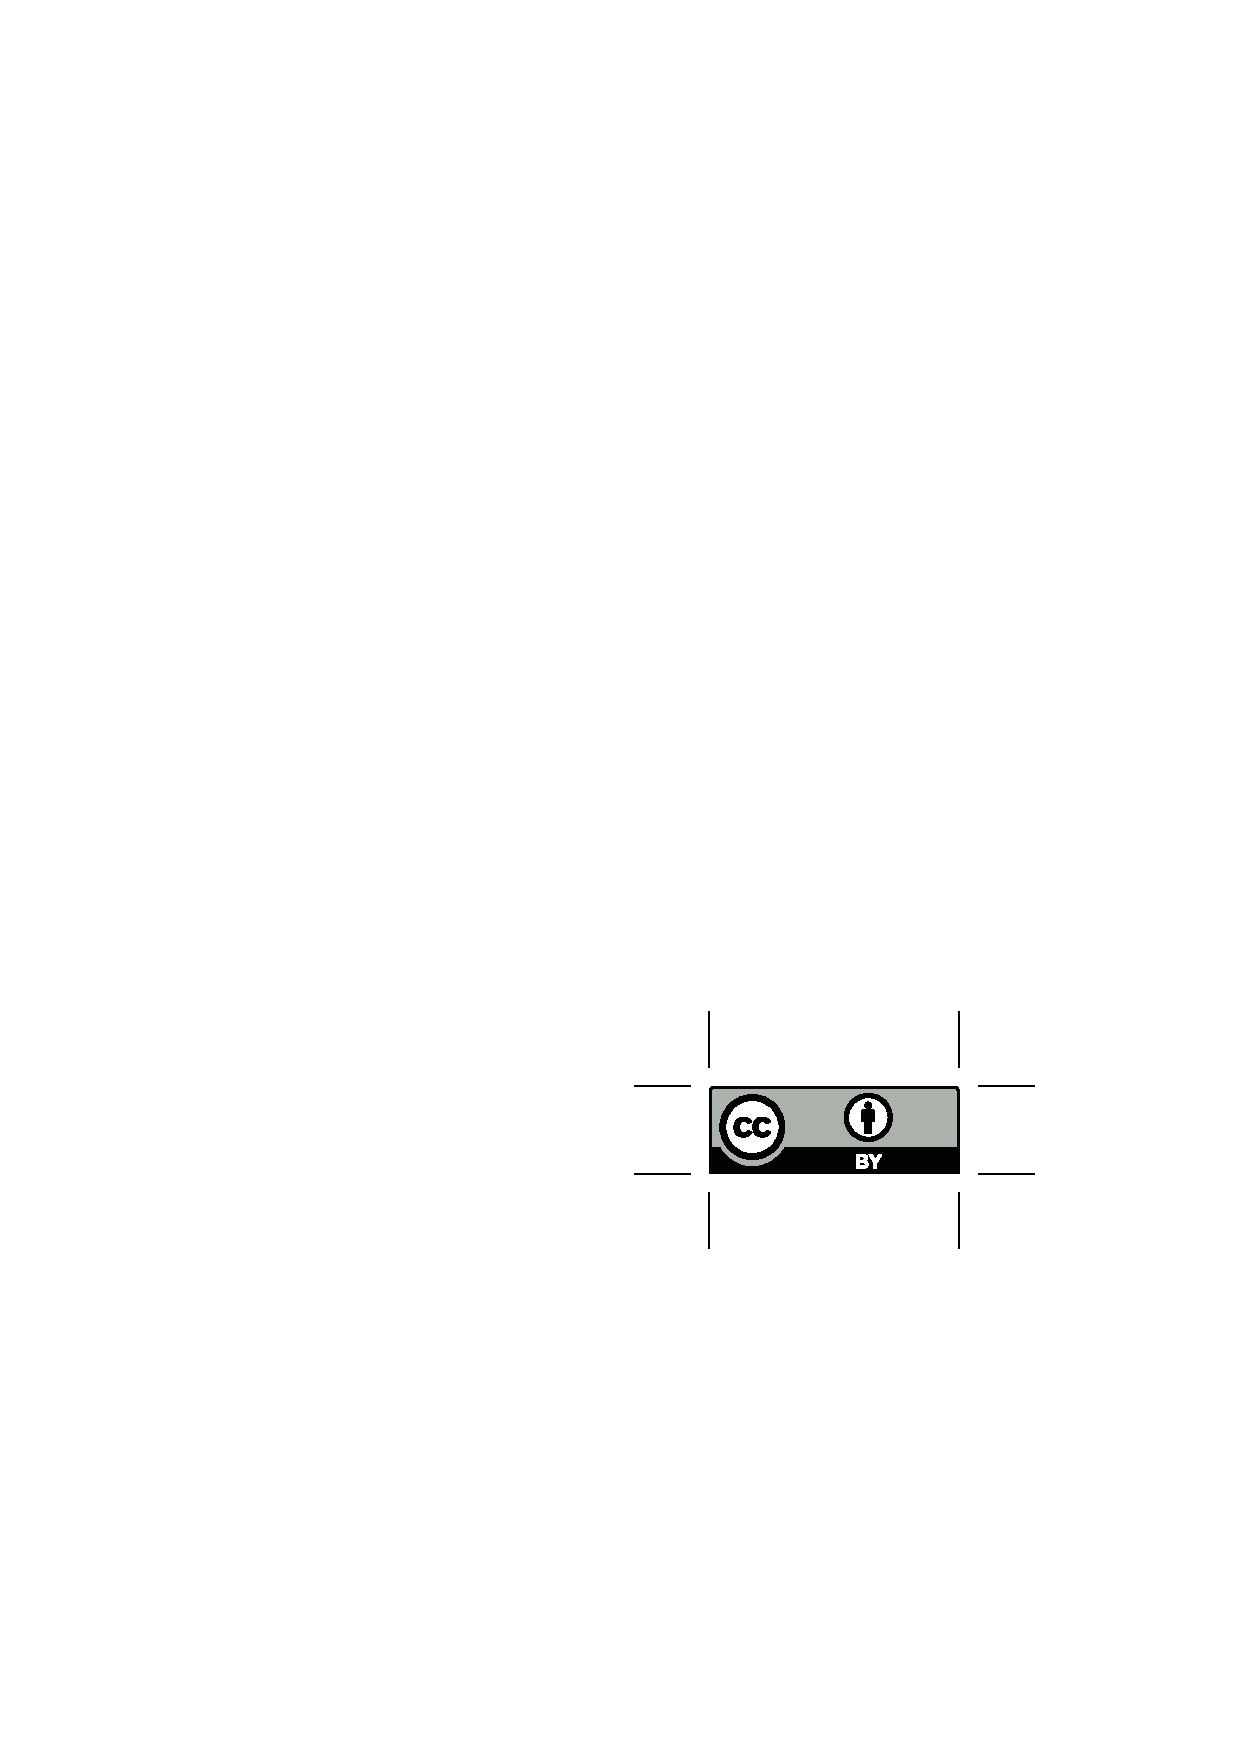
\includegraphics[height=14pt]{by} \\

{\tiny
This work is licensed under a
\href{http://creativecommons.org/licenses/by/4.0/}{Creative Commons Attribution 4.0 International License}.
}}

\begin{document}

\begin{frame}
  \titlepage
\end{frame}

\begin{frame} \frametitle{Divide-and-Conquer}

One of the \emph{big ideas} of computer science problem solving
\begin{enumerate}
  \item \textbf{Divide} a problem into smaller parts
  \item \textbf{Conquer} the smaller problems recursively
  \item \textbf{Combine} the smaller solutions into one solution for the
    original problem
\end{enumerate}

(The term carries some baggage from the age of imperialism.) \stanza

Divide-and-conquer, outside of algorithm design
\begin{itemize}
  \item Software design; breaking features into classes, functions
  \item Networking; OSI seven layer model
  \item Parallel processing; MapReduce
  \item Software process; agile methods; sprints
\end{itemize}

\end{frame}

\begin{frame} \frametitle{Divide-and-conquer at a high level}
  \begin{algorithmic}[1]
    \Function{DIVIDE-AND-CONQUER}{INPUT}
    \If {INPUT is base case}
      \State \Return trivial base case solution
    \Else
      \State $x_1, x_2, \ldots, x_k$ = divide INPUT into $k$ pieces (often 2)
      \State $s_1 = $ DIVIDE-AND-CONQUER($x_1$)
      \State $\ldots$
      \State $s_k = $ DIVIDE-AND-CONQUER($x_k$)
      \State $S$ = combine $s_1, \ldots, s_k$ into one solution
      \State \Return $S$
    \EndIf
    \EndFunction
  \end{algorithmic}
\end{frame}

\begin{frame} \frametitle{Time complexity recurrences}

Recur\underline{sive} pseudocode leads to recu\underline{rrences} in
  run-time functions \stanza

Suppose base case is $n=1$ and takes $\Theta(1)$ time; in the recursive
case we divide evenly into $k$ pieces of size $\approx n/k$, recurse once
on each, and spend $f(n)$ time in the \emph{divide} and \emph{conquer}
phases:
\begin{equation*}
  T(n) = \begin{cases}
          \Theta(1) & \text{ if } n=1, \\
          k T(n/k) + f(n) & \text{ if } n > 1 .
        \end{cases}
\end{equation*}

Recall merge sort divides into $k=2$ pieces, merge takes $\Theta(n)$ time:
\begin{equation*}
  T(n) = \begin{cases}
          \Theta(1) & \text{ if } n=1, \\
          2 T(n/2) + \Theta(n) & \text{ if } n > 1 .
        \end{cases}
\end{equation*}
\end{frame}

\begin{frame} \frametitle{Taking liberties with recurrences}
  General math: bound recurrences precisely including constant factors \stanza

  Algorithm analysis: ordinarily bounding asymptotically; $\Theta$ notation will
    hide constant factors anyway; drop math details that can only impact
    constants and add clutter
  \begin{itemize}
    \item drop ceilings/floors, so write e.g. $n/2$ in lieu of $\lceil n/2 \rceil$ or $\lfloor n/2 \rfloor$
      is more precise
    \item when the base case is $\Theta(1)$ time for $n < c$ for some $c \in \Theta(1)$,
      don't bother writing it explicitly; so
      \begin{equation*}
        T(n) = \begin{cases}
                \Theta(1) & \text{ if } n=1, \\
                2 T(n/2) + \Theta(n) & \text{ if } n > 1 .
              \end{cases}
      \end{equation*}
      is abbreviated as
      \[ T(n) = 2 T(n/2) + \Theta(n) \]
    \end{itemize}

\end{frame}

\begin{frame} \frametitle{Maximum subarray problem}
  \textbf{Maximum subarray problem} \\
  \textbf{input: } an array $\langle p_1, p_2, \ldots, p_n \rangle$ where each
    $p_i \in \mathbb{R}$ is a \emph{profit} (or loss) on day $i$ \\
  \textbf{output: } indices $s, e$ with $s \leq e,$ maximizing the total profit
    \[ \sum_{i=s}^e p_i \]

  Applications
  \begin{itemize}
    \item buy then sell a stock/security
    \item pick opening/closing time of a retail store with slow periods
    \item computer vision, data mining: identify region most consistent with
      a pattern e.g. street striping
  \end{itemize}
\end{frame}

\begin{frame} \frametitle{Examples}
  The optimal subarray may involve negative elements:
  \[ \langle 100, -1, -1, -1, 5, 3 \rangle \]

  Application: when to open/close a cafe:
  \begin{center}
    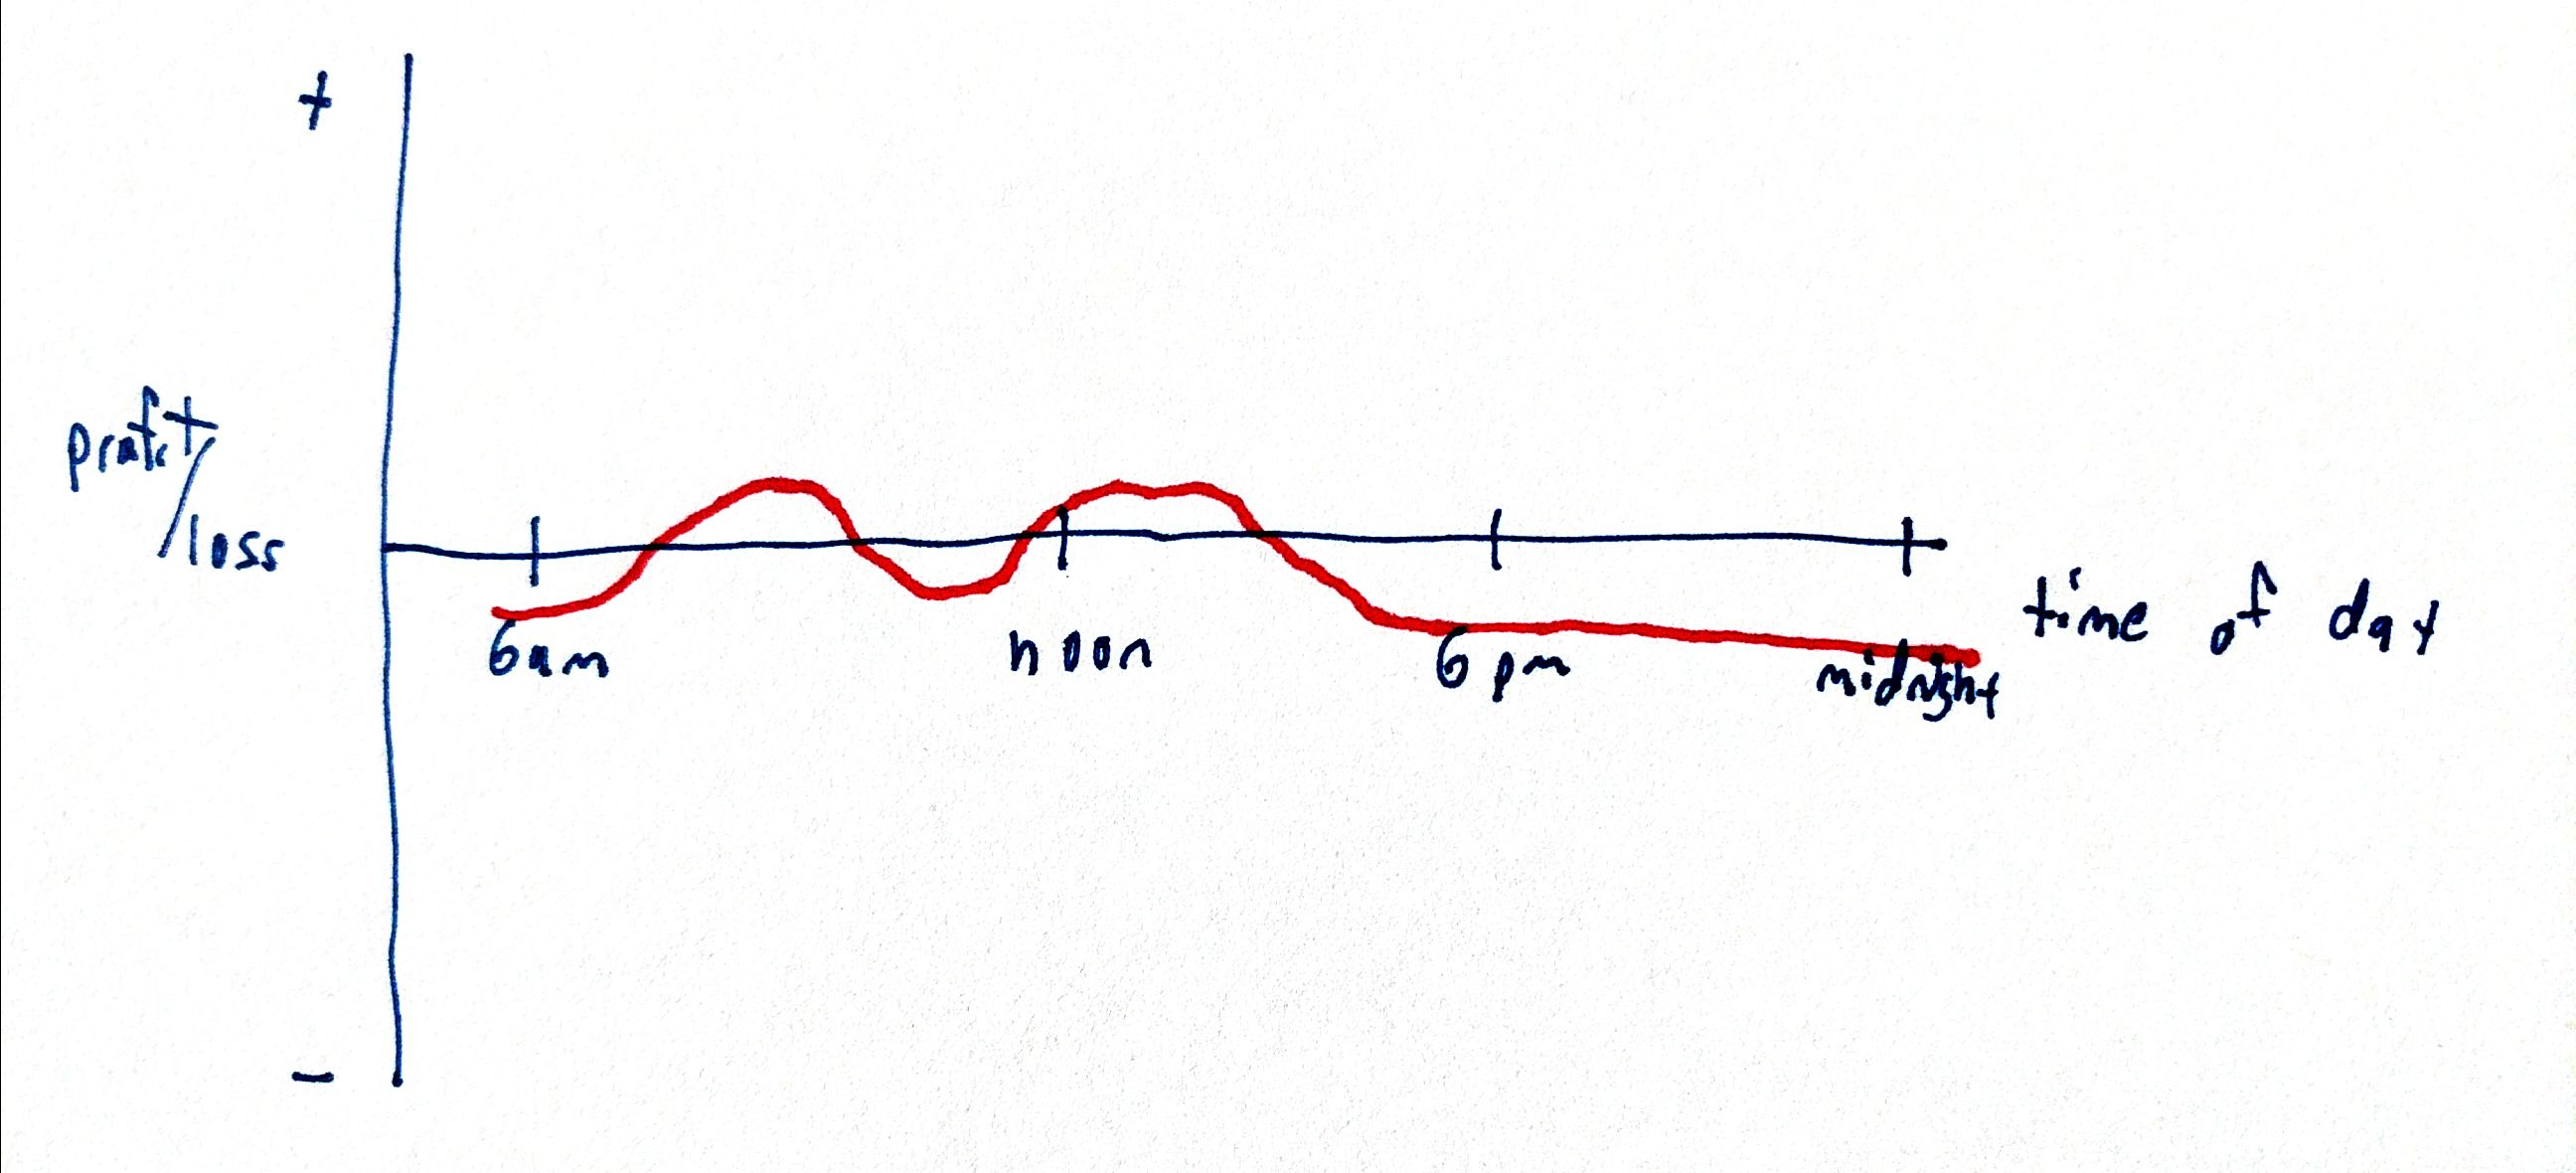
\includegraphics[height=1.5in]{profit-loss.jpg}
  \end{center}
\end{frame}

\begin{frame} \frametitle{Greedy fails}
  Straightforward greedy algorithm would be:
  \begin{itemize}
    \item buy at the lowest price \underline{or} sell at the highest price
    \item incorrect; best "run" could be elsewhere
    \item example: $\langle 0, 1, 10, 4, 4, 4, 4\rangle$
      \begin{itemize}
      \item $\langle 1, 10 \rangle$ is the biggest trough-to-peak; sum 11
      \item but slow-and-steady $\langle 4, 4, 4, 4\rangle$ has sum 12
        \end{itemize}
    \item not always correct $\implies$ not actually an algorithm
  \end{itemize}

\end{frame}

\begin{frame} \frametitle{Brute force}
  Exhaustive search: try every legal start/end

  \begin{algorithmic}[1]
    \Function{BRUTE-FORCE-MAX-SUBARRAY}{P}
    \State $s = e = 1$
    \For {$i$ from 1 to $n$}
      \For {$j$ from $i$ to $n$}
        \If {$(\sum p_i \ldots p_j) > (\sum p_s \ldots p_e)$}
          \State $s=i, e=j$
        \EndIf
      \EndFor
    \EndFor
    \State \Return $(s, e)$
    \EndFunction
  \end{algorithmic}

  $\Theta(n^3)$ time as written; can cache sums to achieve
  $\Theta(n^2)$

\end{frame}

\begin{frame} \frametitle{Divide-and-conquer brainstorm}
\textbf{Divide:} chop array in half into two smaller arrays $L, R$\\
\textbf{Conquer:} recursively compute maximum subarray in $L$ and in $R$ \\
\textbf{Combine:} maximum subarray of entire $P$ could be
\begin{enumerate}
  \item subarray entirely in $L$;
  \item subarray entirely in $R$; or
  \item \emph{crossing} subarray that starts in $L$ and ends in $R$
\end{enumerate}
(exhaustive case analysis)

Theme with \textbf{combine}: choose best among small solutions (easy) or
a distinct solution that crosses boundaries (trickier)
\end{frame}

\begin{frame} \frametitle{Identify crossing subarray --- try 1}
Suppose the two pieces of $P$ are $P[low \ldots mid]$ and
  $P[mid+1 \ldots high]$ \stanza

Tempting to try all pairs of $s \in \{low, \ldots, mid \}$ and
$e \in \{mid+1, \ldots, high\}$ \stanza

Would work, but
\begin{itemize}
  \item time becomes $T(n) = 2 T(n/2) + \Theta(n^2)$ which is $\Theta(n^2)$
    by master theorem
  \item same time as brute force, but more complicated $\implies$ not a win
\end{itemize}
\end{frame}

\begin{frame} \frametitle{Identify crossing subarray --- insight}
Theme in algorithm design: in general, a more specific problem admits a
  faster and/or simpler algorithm \stanza

First try is not using the fact that a \emph{crossing} subarray
\underline{must} cross $mid$
\begin{itemize}
  \item substantially simplifies the search
  \item $s$ is how far before $mid$; \underline{separately}, $e$ is how far after $mid$?
  \item two separate 1D searches $\implies$ two linear loops
  \item $\Theta(n)+\Theta(n) = \Theta(2n) = \Theta(n)$ time
  \item versus: $s$ is where, and $e$ is how much later?
  \item 2D search $\implies$ two nested loops $\implies \Theta(n^2)$ time
  \item location of the "2" is profound; $\Theta(2n) \ll \Theta(n^2)$
\end{itemize}
\end{frame}

\begin{frame} \frametitle{Identify crossing subarray --- try 2}
\begin{columns}
\begin{column}{0.6\textwidth}
  {\tiny
  \begin{algorithmic}[1]
    \Function{MAX-CROSSING-SUBARRAY}{P, low, mid, high}
    \State $leftsum = rightsum = -\infty$
    \State $sum = 0$
    \For {$i$ from $mid$ down to $low$}
      \State $sum = sum + P[i]$
      \If { $sum > leftsum$ }
        \State $leftsum = sum$
        \State $maxleft = i$
      \EndIf
    \EndFor
    \State $sum = 0$
    \For {$i$ from $mid+1$ to $high$}
      \State $sum = sum + P[i]$
      \If { $sum > rightsum$ }
        \State $rightsum = sum$
        \State $maxright = i$
      \EndIf
    \EndFor
    \State \Return $(maxleft, maxright, leftsum + rightsum)$
    \EndFunction
  \end{algorithmic}
  }
\end{column}
\begin{column}{0.4\textwidth}
  $\Theta(n)$ time \stanza

  (Note scoping of $maxleft, maxright$, and that they are inevitably initialized.)
\end{column}
\end{columns}
\end{frame}

\begin{frame} \frametitle{Maximum subarray algorithm}
  {\tiny
  \begin{algorithmic}[1]
    \Function{MAX-SUBARRAY}{P, low, high}
    \If { $low$ == $high$ }
      \State \Return $(low, high, P[low])$
    \Else
      \State $mid = \lceil (low+high)/2 \rceil$
      \State $(leftlow, lefthigh, leftsum) = MAX-SUBARRAY(P, low, mid)$
      \State $(rightlow, righthigh, rightsum) = MAX-SUBARRAY(P, mid+1, high)$
      \State $(crosslow, crosshigh, crosssum) = MAX-CROSSING-SUBARRAY(A, low, mid, high)$
      \If { $leftsum \geq rightsum \text{ and } leftsum \geq crosssum$ }
        \State \Return $(leftlow, lefthigh, leftsum)$ \Comment{ entirely-left subarray}
      \ElsIf { $rightsum \geq leftsum \text{ and } rightsum \geq crosssum$ }
        \State \Return $(rightlow, righthigh, rightsum)$ \Comment{ entirely-right subarray }
      \Else
        \State \Return $(crosslow, crosshigh, crosssum)$ \Comment{ mid-crossing subarray }
      \EndIf
    \EndIf
    \EndFunction
  \end{algorithmic}
  }
\end{frame}

\begin{frame} \frametitle{Maximum subarray analysis}
  D\&C runtime is \[ T(n) = 2 T(n/2) + \Theta(n) \]

  Solves to $\Theta(n \log n)$, by master theorem, same as merge sort. \stanza

  Brute force was $\Theta(n^2)$
  \begin{itemize}
    \item D\&C is much faster
    \item perhaps counterintuitive due to recursion's reputation for sloth
    \item D\&C benefits from observation that subarrays are contiguous, so
      extend in two directions from a middle
    \item brute force is oblivious to this
    \item human mathematical insight eliminates wasted effort
  \end{itemize}
\end{frame}

\begin{frame} \frametitle{Matrix multiplication}
  \textbf{Matrix multiplication problem} \\
  \textbf{input: } $A, B$ each an $n \times n$ matrix \\
  \textbf{output: } matrix product $C = AB$ \stanza

  Recall notation: element at row $i$ and column $j$ of matrix $A$ is
  denoted $a_{ij}$ \stanza

  Definition of matrix multiplication:
  \[ c_{ij} = \sum_{k=1}^n a_{ik} \cdot b_{kj} . \]
\end{frame}

\begin{frame} \frametitle{Na\"ive matrix multiplication}
  {
  \begin{algorithmic}[1]
    \Function{MATRIX-MULTIPLY}{A, B}
    \State $C = $ new $n \times n$ matrix
    \For { $i$ from 1 to $n$ }
      \For { $j$ from 1 to $n$ }
        \State $c_{ij} = 0$
        \For { $k$ from 1 to $n$ }
          \State $c_{ij} = c_{ij} + a_{ik} \cdot b_{kj}$
        \EndFor
      \EndFor
    \EndFor
    \State \Return $C$
    \EndFunction
  \end{algorithmic}
  }
  $\Theta(n^3)$ time
\end{frame}

\begin{frame} \frametitle{Is na\"ive optimal?}
The definition of matrix multiplication involves a sum that is iterated $n$
times, for each of the $n \times n$ elements of $C$, which might seem to
require exactly $n^3$ scalar multiply instructions, and imply an
$\Omega(n^3)$ lower bound for matrix multiplication. \stanza

\textbf{Surprise!} Strassen's algorithm (1969) takes $O(n^{\lg 7})=O(n^{2.81})$ time;
 more complicated Williams-Le Gall algorithm (2014) takes $O(n^{2.37})$ time \stanza

\emph{Insight:} per the definition of matrix multiplication, some elements of
$A$ and $B$ are multiplied together more than once; avoid duplicating these
efforts.
\end{frame}

\begin{frame} \frametitle{Moving to divide-and-conquer}
  Suppose $n$ is an even power of 2, i.e. $n=2^k$ for $k \geq 0$ \\
  (Can preprocess $A, B$ by adding padding zeroes, then trim the zeroes
   out of $C.$)

  Divide $A$ into four equal-size submatrices, and same for $B, C$.
  \[ A = \begin{bmatrix} A_{11} & A_{12} \\ A_{21} & A_{22} \end{bmatrix},
     B = \begin{bmatrix} B_{11} & B_{12} \\ B_{21} & B_{22} \end{bmatrix},
     C = \begin{bmatrix} C_{11} & C_{12} \\ C_{21} & C_{22} \end{bmatrix},
   \]
  so we can compute $C$ as
  \[ \begin{bmatrix} C_{11} & C_{12} \\ C_{21} & C_{22} \end{bmatrix}
     =
     \begin{bmatrix} A_{11} & A_{12} \\ A_{21} & A_{22} \end{bmatrix}
     \cdot
     \begin{bmatrix} B_{11} & B_{12} \\ B_{21} & B_{22} \end{bmatrix} . \]
\end{frame}

\begin{frame} \frametitle{Moving to divide-and-conquer (continued)}
\[ \begin{bmatrix} C_{11} & C_{12} \\ C_{21} & C_{22} \end{bmatrix}
   =
   \begin{bmatrix} A_{11} & A_{12} \\ A_{21} & A_{22} \end{bmatrix}
   \cdot
   \begin{bmatrix} B_{11} & B_{12} \\ B_{21} & B_{22} \end{bmatrix} \]
can be broken down into four separate computations
\begin{align*}
  C_{11} &= A_{11} \cdot B_{11} + A_{12} \cdot B_{21} \\
  C_{12} &= A_{11} \cdot B_{12} + A_{12} \cdot B_{22} \\
  C_{21} &= A_{21} \cdot B_{11} + A_{22} \cdot B_{21} \\
  C_{22} &= A_{21} \cdot B_{12} + A_{22} \cdot B_{22} \\
\end{align*}
each of which can be performed recursively.
\end{frame}

\begin{frame} \frametitle{Divide-and-conquer matrix multiplication --- try 1}
  {
  \begin{algorithmic}[1]
    \Function{MMR}{A, B}
    \State $C = $ new $n \times n$ matrix
    \If { $n$ == 1 }
      \State $c_{11} = a_{11} \cdot b_{11}$
    \Else
      \State quadrisect $A, B, C$
      \State $C_{11} = MMR(A_{11}, B_{11}) + MMR(A_{12}, B_{21})$
      \State $C_{12} = MMR(A_{11}, B_{12}) + MMR(A_{12}, B_{22})$
      \State $C_{21} = MMR(A_{21}, B_{11}) + MMR(A_{22}, B_{21})$
      \State $C_{22} = MMR(A_{21}, B_{12}) + MMR(A_{22}, B_{22})$
    \EndIf
    \State \Return $C$
    \EndFunction
  \end{algorithmic}
  }
\end{frame}

\begin{frame} \frametitle{Analysis}
\begin{itemize}
  \item each of the submatrices $A_{11},$ etc. has size $n/2$
  \item quadrisecting $A, B$ is $\Theta(n^2)$ time; same for assembling $C$
  \item each matrix $+$ takes $\Theta( (\frac{n}{2})^2 ) = \Theta(\frac{n^2}{4}) = \Theta(n^2)$ time
  \item 8 recursive calls
\end{itemize}
\[ T(n) = 8 T(n/2) + \Theta(n^2) \]

Solves to $T(n) \in \Theta(n^3)$ by master theorem; same as na\"ive \stanza

Observe: the 8 factor is meaningful, but the $\frac{1}{4}$ isn't \\
$\implies$ it's a win to have fewer recursive calls, but more work (by a
constant factor) in the \textbf{combine} step
\end{frame}

\begin{frame} \frametitle{Strassen's insight}
Use algebra to refactor into 7 recursive multiplies instead of 8
\begin{enumerate}
  \item quadrisect $A, B, C$ as before
  \item create 10 $(n/2) \times (n/2)$ submatrices $S_1, \ldots, S_{10}$ using
    matrix + and -
  \item recursively compute 7 submatrix products $P_1, \ldots, P_7$ in terms of
    the matrices from steps 1, 2
  \item compute $C_{11}, C_{12}, C_{21}, C_{22}$ using matrix + and -
\end{enumerate}
\begin{align*}
  T(n) &= \Theta(n^2) + \Theta(10 \frac{n}{4}) + 7 T(n/2) + T(4 \frac{n}{4}) \\
       &= 7 T(n/2) + \Theta(n^2) \\
       &\in \Theta(n^{\lg 7})
\end{align*}
by master theorem
\end{frame}
\begin{frame} \frametitle{Divide-and-conquer matrix multiplication --- try 2}
  {\tiny
  \begin{algorithmic}[1]
    \Function{MMS}{A, B}
    \State $C = $ new $n \times n$ matrix
    \If { $n$ == 1 }
      \State $c_{11} = a_{11} \cdot b_{11}$
    \Else
      \State quadrisect $A, B, C$
      \State form $S_1, \ldots, S_{10}$ as shown on next slide
      \State $P_1 = MMS(A_{11}, S_1)$
      \State $P_2 = MMS(S_2, B{22})$
      \State $P_3 = MMS(S_3, B{11})$
      \State $P_4 = MMS(A_{22}, S_4)$
      \State $P_5 = MMS(S_5, S_6)$
      \State $P_6 = MMS(S_7, S_8)$
      \State $P_7 = MMS(S_9, S_{10})$
      \State $C_{11} = P_5 + P_4 - P_2 + P_6$
      \State $C_{12} = P_1 + P_2$
      \State $C_{21} = P_3 + P_4$
      \State $C_{22} = P_5 + P_1 - P_3 - P_7$
    \EndIf
    \State \Return $C$
    \EndFunction
  \end{algorithmic}
  }
\end{frame}


\begin{frame} \frametitle{Details of Strassen's algorithm}
  \begin{columns}
  \begin{column}{0.5\textwidth}
    \begin{align*}
      S_1    &= B_{12} - B_{22} \\
      S_2    &= A_{11} + A_{12} \\
      S_3    &= A_{21} + A_{22} \\
      S_4    &= B_{21} - B_{11} \\
      S_5    &= A_{11} + A_{22} \\
      S_6    &= B_{11} + B_{22} \\
      S_7    &= A_{12} - A_{22} \\
      S_8    &= B_{21} + B_{22} \\
      S_9    &= A_{11} - A_{21} \\
      S_{10} &= B_{11} + B_{12} \\
    \end{align*}
  \end{column}
  \begin{column}{0.5\textwidth}
    \begin{align*}
      P_1 &= A_{11} \cdot S_1 \\
      P_2 &= S_2 \cdot B_{22} \\
      P_3 &= S_3 \cdot B_{11} \\
      P_4 &= A_{22} \cdot S_4 \\
      P_5 &= S_5 \cdot S_6 \\
      P_6 &= S_7 \cdot S_8 \\
      P_7 &= S_9 \cdot S_{10} \\
      C_{11} &= P_5 + P_4 - P_2 + P_6 \\
      C_{12} &= P_1 + P_2 \\
      C_{21} &= P_3 + P_4 \\
      C_{22} &= P_5 + P_1 - P_3 - P_7 \\
    \end{align*}
  \end{column}
 \end{columns}
\end{frame}

\begin{frame} \frametitle{Editorial Commentary}
\begin{itemize}
  \item proof that 7 recursive multiplies suffice, instead of 8, is surprising
    and therefore interesting
  \item equations on previous slide are relatively uninteresting (though not
    unimportant) \textbf{technical detail}
  \item $o(n^3)$ matrix multiply is of great theoretical interest (because
    surprise)
  \item but the na\"ive alg. has substantially better constant factors, and
    the gap between $\Theta(n^3)$ and $\Theta(n^{2.81})$ is narrow
  \item Strassen (and descendants) are only practical for very large $n$
  \item in practice: na\"ive alg. for base case $n<128$ (say)
\end{itemize}
\end{frame}

\begin{frame} \frametitle{Takeaways}
Recall
\begin{itemize}
  \item insertion sort is $\Theta(n^2)$; D\&C merge sort is $\Theta(n \log n)$
  \item brute force maximum subarray is $\Theta(n^2)$; D\&C alg. is $\Theta(n \log n)$
  \item na\"ive matrix multiply is $\Theta(n^3)$; Strassen's alg. is $\Theta(n^{2.81})$
\end{itemize}
In each case study,
\begin{itemize}
  \item first try was no faster; just using D\&C isn't an automatic improvement
  \item master method analyses hinted at the bottleneck
  \item shift work around to decrease asymptotic time complexity (but increase
    constant factors); beneficial trade-off
  \item optimization comes from human insight into the problem
  \item unclear how to make these insights w/o the D\&C framing
\end{itemize}
\end{frame}

\begin{frame} \frametitle{Master Method}
  \begin{itemize}
    \item \textbf{Master method:} plug-and-chug process for solving some recurrences
    \begin{itemize}
      \item doesn't work for \emph{all}
      \item but works for \emph{typical} D\&C recurrences
    \end{itemize}
  \item \textbf{Master theorem:} proof that the method is sound
  \end{itemize}
\end{frame}

\begin{frame} \frametitle{Master Theorem}
Let $a \geq 1, b>1$ be constants, $f(n)$ be a function, and $T(n)$ be the recurrence
\[ T(n) = a T(n/b) +f(n) . \]
Then
\begin{enumerate}
  \item If $\exists \epsilon>0$ such that $f(n) = O(n^{log_b a-\epsilon}),$ then $T(n)=\Theta(n^{\log_b a}).$
  \item If $f(n) = O(n^{log_b a}),$ then $T(n)=\Theta(n^{\log_b a} \log n).$
  \item If $\exists \epsilon>0$ such that $f(n) = \Omega(n^{log_b a+\epsilon}),$
    and $a f(n/b) \leq cf(n)$ for some $c<1$ and sufficiently large $n,$
    then $T(n)=\Theta(f(n)).$
\end{enumerate}
\end{frame}

\begin{frame} \frametitle{Step 1: Identify Relevant Case}
  3 cases: $f(n)$ is asymptotically
  \begin{enumerate}
    \item less than,
    \item equal,
    \item greater than
  \end{enumerate}
  the benchmark $ n^{\log_b a} .$
  \vspace{10pt}

  So identify $a$ and $b,$ substitute into $n^{\log_b a},$ simplify, and decide among the cases.
  \vspace{10pt}

  If unsure, take the limit
  \[ \lim_{n \rightarrow \infty} \frac{f(n)}{n^{\log_b a}} . \]
\end{frame}

\begin{frame} \frametitle{Step 1: Identify Relevant Case}
  Example:
  \[ T(n) = 2 T(n/2) + 7 \]

  Identify: $a=2,$ $b=2$

  Plug and chug:
  \[ n^{\log_b a} = n^{\log_{(2)} (2)} = n^{(1)} = n \]

  Is $7$ less than, equal, or greater than $n$? \vspace{10pt}

  Intuition: less than \vspace{10pt}

  Check:
  \[ \lim_{n \rightarrow \infty} \frac{7}{n} = 0 \]
 \end{frame}

 \begin{frame} \frametitle{Step 2 alternative 1: Justify Case 1}
  Need to Prove: If $\exists \epsilon>0$ such that $f(n) = O(n^{log_b a-\epsilon}),$ then $T(n)=\Theta(n^{\log_b a}).$
  \vspace{10pt}

  Prove by showing an example of a $\epsilon$ that makes $f(n) = O(n^{log_b a-\epsilon}).$
  \vspace{10pt}

  Continuing example: show $\epsilon$ s.t. $7 = O(n^{1-\epsilon})$
  Choose $\epsilon=1,$ so we have $7=O(n^{1-(1)}) = O(n^0) = O(1)$
  \vspace{10pt}

  Justification: ``We have $f(n)=7$ and $n^{\log_b a} = n^{\log_{(2)} (2)} = n^{(1)} = n.$ Let $\epsilon=1;$
  then $f(n) = O(n^{\log_b a - \epsilon}) = O(n^{(1)-(1)}) = O(n^{(0)}) = O(1)$, and by case 1 of the master theorem,
  $T(n) = \Theta(n^{\log_b a}) = \Theta(n).$''

\end{frame}

 \begin{frame} \frametitle{Step 2 alternative 2: Justify Case 2}
  Need to Prove: If $f(n) = O(n^{\log_b a}),$ then $T(n)=\Theta(n^{\log_b a} \log n).$
  \vspace{10pt}

  Case 2 is true without qualification; don't need to show anything else.
  \vspace{10pt}

  Example: $T(n) = 2T(n/2) + 5n,$ so $a=2,$ $b=2,$ and $f(n)=5n.$
  \vspace{10pt}

  $n^{\log_b a} = n^{\log_{(2)} (2)} = n^{(1)} = n$ is asymptotically equal to $f(n)=5n$ so case 2 applies
  and $T(n)=\Theta(n^{\log_b a} \log n) = \Theta(n \log n).$
  \vspace{10pt}

 Justification: ``We have $f(n)=5n$ and $n^{\log_b a} = n^{\log_{(2)} (2)} = n^{(1)} = n.$ Case 2 of the
 master theorem applies, so $T(n)=\Theta(n^{\log_b a} \log n) = \Theta(n^{(1)} \log n) = \Theta(n \log n).$ ''
 \end{frame}


 \begin{frame} \frametitle{Step 2 alternative 3: Justify Case 3}
  Need to Prove: If $\exists \epsilon>0$ such that $f(n) = \Omega(n^{log_b a+\epsilon}),$
  and $a f(n/b) \leq cf(n)$ for some $c<1$ and sufficiently large $n,$
  then $T(n)=\Theta(f(n)).$
  \vspace{10pt}

  Prove by showing examples of $\epsilon, c$ that makes $f(n) = O(n^{log_b a+\epsilon})$
  and $a f(n/b) \leq cf(n)$ for large $n$.
  \vspace{10pt}

  Example: $T(n) = 2T(n/2) + n^2,$ so $a=2,$ $b=2,$ and $f(n)=n^2.$
  \vspace{10pt}

  $n^{\log_b a} = n^{\log_{(2)} (2)} = n^{(1)} = n.$ Can choose $\epsilon=1$ to have $\Omega(n^{1+(1)}).$
  \vspace{10pt}
\end{frame}

\begin{frame} \frametitle{Step 2 alternative 3: Justify Case 3 (cont'd)}
  Need
  \begin{align*}
    a f(n/b) &\leq cf(n) \\
    (2) f(\frac{n}{2}) &\leq c(n^2) \\
    2 \cdot (\frac{n}{2})^2 &\leq c n^2 \\
    2 \cdot \frac{n^2}{4} &\leq c n^2 \\
    \frac{1}{2} &\leq c \\
  \end{align*}

  Any $c \geq \frac{1}{2}$ can work; arbitrarily choose $c=1.$
\end{frame}

\begin{frame} \frametitle{Step 2 alternative 3: Justify Case 3 (cont'd)}
 Justification: ``We have $f(n)=n^2$ and $n^{\log_b a} = n^{\log_{(2)} (2)} = n^{(1)} = n.$
 Let $\epsilon=1;$
  then $f(n) = \Omega(n^{\log_b a + \epsilon}) = \Omega(n^{(1)+(1)}) = \Omega(n^2).$
 Let $c=1;$ then
  $af(n/b) = (2)f(n/(2)) = 2(n/2)^2 = 2(n^2/4) = n^2/2 \leq cf(n) = (2)n^2$ for sufficiently large $n$.
  Case 3 of the master theorem applies, so $T(n)=\Theta(f(n)) = \Theta(n^2).$ ''
 \end{frame}

 \begin{frame} \frametitle{Limitations Of The Master Method}
  Master Theorem is a big ``if/then''
  \vspace{10pt}

Theorem does not apply when:
\begin{itemize}
  \item $T(n)$ not in the necessary form, or
  \item none of cases 1, 2, 3 apply
\end{itemize}
\vspace{10pt}

There are gaps between the cases.
\vspace{10pt}

\textbf{However,} when an algo. is designed according to the D\&C pattern, the master theorem almost always applies.

\end{frame}
 
\end{document}
